\chapter{Design}
\section*{Introduction}
After identifying the functional and non-functional needs and the main functionalities of our application. We begin this part
of the conceptual study by describing the general architecture of our system and
its detailed internal modeling through class and sequence diagrams.
\section{Global Architecture}
In this section, we will give an overview of the definition of the
the architectural pattern was chosen to model our application and we will
detail the projection of this pattern on our application.
\subsection{Definition of the Clean Architecture pattern}
Clean architecture is a software design philosophy proposed by Robert C. Martin, aka Uncle Bob. This architecture is based on:
\begin{itemize}
\item The SOLID principles from which derive the principle of inversion of control and the
principle of dependency injection (a framework external to the application
creates the components of the application and injects the dependencies between these
components
\item The principle of separation of "business rules" (independent of the applications) and the "application rules".
\item The principle of independence from the core of the application of necessary technologies
 for its operation.
\end{itemize}
Thanks to these principles, the components of the application become easy to
manage, test, modify and reuse.\\
The clean architecture pattern is divided into 4 layers (upcoming figure) whose meaning
dependency is incoming:
\begin{itemize}
\item \textbf{Entities}\\
Entities that represent application domain objects with
their methods (Business Rules).
\item \textbf{Use Cases}\\
This layer represents the logic of the application, i.e. the rules
specific to an application (Application Rules).
\item \textbf{Inerfaces / Adapters}\\
This layer represents the interface between systems external to the application (framework, databases, UI...) and the core of the application (entities +
use case). This layer allows formatting, structuring, and adaptation of incoming and outgoing data.
\item \textbf{External technologies}\\
This layer represents the layer external to the application grouping the
technologies necessary for its operation (APIs, frameworks, Databases, UI, network, drivers, devices, etc.).
\end{itemize}
\begin{figure}[H]%
    \center   
    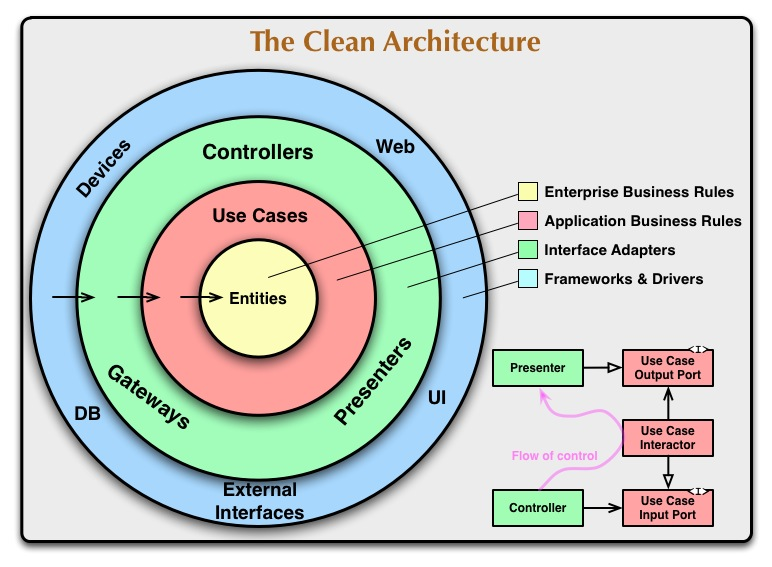
\includegraphics[scale=0.5]{clean.jpg}
    \caption{Clean Architecture}
\end{figure}
\subsection{Application of the "Clean Architecture" pattern}
We explain in this paragraph the details of the projection of the pattern
Clean Architecture on our app.\\
The following figure represents the class diagram which illustrates the binding
between entities (classes). Indeed, this diagram translates the content of the \textbf{Entities} layer.
\begin{figure}[H]%
    \center   
    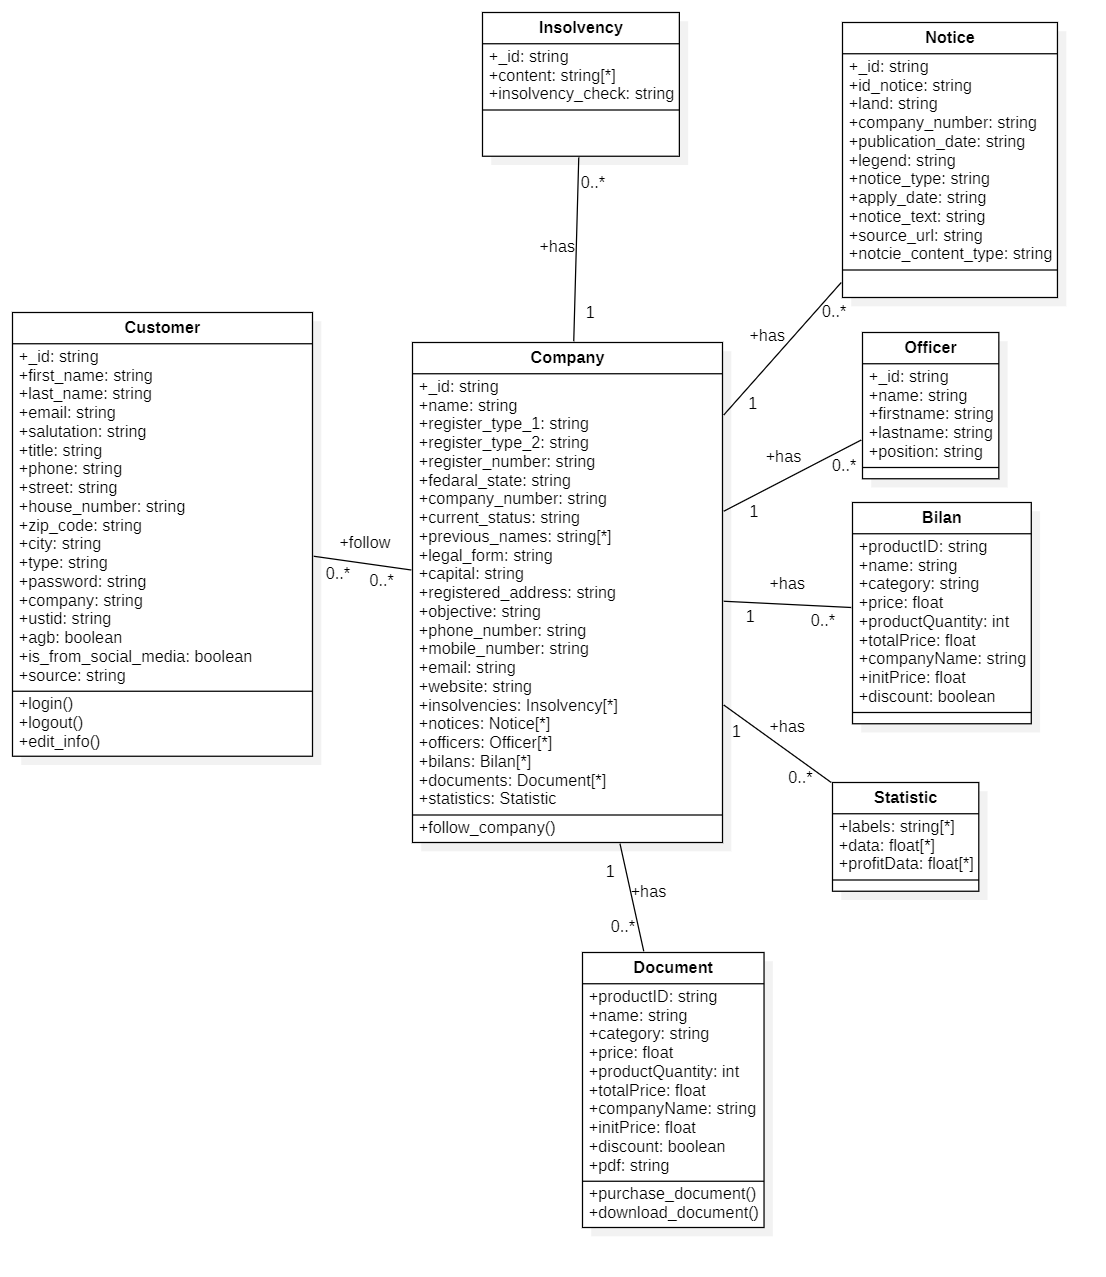
\includegraphics[scale=0.45]{class.png}
    \caption{Class diagram representing the "Entities" layer}
\end{figure}
\newpage
Description of classes representing our entities:
\begin{itemize}
\item \textbf{Customer:}\\
This class represents our application's customers who may log in, log out, and edit their account information. This class's attributes are:
\begin{itemize}
\item[•] \_ id: the identifier of the customer
\item[•] first\_ name: the first name of the customer
\item[•] last\_ name: the last name of the customer
\item[•] email: the email of the customer
\item[•] salutation: the salutation of the customer ( Herr, Frau)
\item[•] title: the title of the customer ( Prof., Dr.)
\item[•] phone: the phone number of the customer
\item[•] street: the street part of the customer's address
\item[•] house\_ number: the house number part of the customer's address
\item[•] zip\_ code: the zip code part of the customer's address
\item[•] city: the city part of the customer's address
\item[•] password: the password of the customer
\item[•] company: the company of the customer
\item[•] ustid: the value-added tax identification number (VAT ID) of the customer's company if he has one
\item[•] agb: boolean variable presenting if the customer has accepted the agreements of the platform
\item[•] is\_ from\_ social\_ media: boolean variable presenting if the customer's account was created using a social media account
\item[•] source: the social media of the customer account (Facebook, Google, LinkedIn, Xing, empty value)
\end{itemize}
\item \textbf{Company:}\\
This class represents the companies in our application that can be followed by the customer. This class's attributes are:
\begin{itemize}
\item[•] \_ id: the identifier of the company
\item[•] name: the latest name of the company
\item[•] register\_ type\_ 1: the first part of the company's German type
\item[•] register\_ type\_ 2: the second part of the company's German type
\item[•] register\_ number: the German commercial register number of the company
\item[•] federal\_ state: the German federal state name of the company
\item[•] company\_ number: the number of the company in our database
\item[•] current\_ status: the current status of the company ( active, shutdown)
\item[•] prevoius\_ names: list of the company's previous names
\item[•] legal\_ form: the legal form of the company (GmbH, Limited \& Co. KG, etc)
\item[•] capital: the capital of the company in euros
\item[•] registerd\_ address: the latest address of the company
\item[•] objective: the objective of the company
\item[•] phone\_ number: the latest phone number of the company
\item[•] mobile\_ number: the latest mobile phone number of the company
\item[•] email: the latest email of the company
\item[•] website: the latest website of the company
\item[•] insolvencies: list of the company's insolvencies notices
\item[•] notices: list of the company's change notices
\item[•] officers: list of the company's office workers and individuals
\item[•] bilans: list of the company's balance sheets
\item[•] documents: list of the company's available purchasable documents
\item[•] statistics: visualization data of the company's business performance 


\end{itemize}
\item \textbf{Insolvency}\\
This class presents the insolvencies notices in our application. This class's attributes are:
\begin{itemize}
\item[•] \_ id: the identifier of the company's insolvencies
\item[•] content: the list of notices from the company
\item[•] insolvency\_ check: variable representing if the company has a bad record in insolvencies ( positive, negative)
\end{itemize}
\item \textbf{Notice}\\
This class presents the change notices in our application. This class's attributes are:
\begin{itemize}
\item[•] \_ id: the identifier of the notice
\item[•] id\_ notice: the identifier of the notice regarding each company
\item[•] land: the location of the release of the notice
\item[•] company\_ number: the number of the company owning the notice
\item[•] publication\_ date: the date of publication of the notice
\item[•] legend: the label of the notice
\item[•] notice\_ type: the type of the notice
\item[•] apply\_ date: the date of application of the notice
\item[•] notice\_ text: the content of the notice
\item[•] source\_ url: the source of the notice
\item[•] notice\_ content\_ type: the type content of the notice
\end{itemize}
\item \textbf{Officer}\\
This class presents the officer(office worker/individuals) in our application. This class's attributes are:
\begin{itemize}
\item[•] \_ id: the identifier of the officer

\item[•] name: the full name of the officer
\item[•] firstname: the first name of the officer
\item[•] lastname: the last name of the officer
\item[•] position: the position of the officer

\end{itemize}
\item \textbf{Bilan}\\
This class presents the balance sheets in our application. This class's attributes are:
\begin{itemize}
\item[•] productID: the identifier of the sheet

\item[•] name: the name of the sheet
\item[•] category: the category of the sheet
\item[•] price: the price of the sheet
\item[•] productQuantity: the available quantity of the sheet
\item[•] totalPrice: the full price of the sheet
\item[•] companyName: the name of the company owning the sheet
\item[•] initPrice: the initial price of the sheet
\item[•] discount: boolean variable presenting if the sheet is on discount
\end{itemize}
\item \textbf{Statistic}\\
This class presents the statistics data in our application. This class's attributes are:
\begin{itemize}
\item[•] labels: the values on the X axis on the graph ( usually year values) 

\item[•] data: the values on the Y axis on the graph ( usually turnover values) 
\item[•] profitData: the data for profit values on the graph


\end{itemize}

\item \textbf{Documents}\\
This class presents documents in our application, the customer can purchase these documents and download them as pdf files once purchased. This class's attributes are:
\begin{itemize}
\item[•] productID: the identifier of the document

\item[•] name: the name of the document
\item[•] category: the category of the document
\item[•] price: the price of the document
\item[•] productQuantity: the available quantity of the document
\item[•] totalPrice: the full price of the document
\item[•] companyName: the name of the company owning the document
\item[•] initPrice: the initial price of the document
\item[•] discount: boolean variable presenting if the document is on discount
\item[•] pdf: the link to the pdf file corresponding to the document
\end{itemize}
\end{itemize}
%End of page 35 in the Selma report%
The classes we have defined in the "Entities" layer are related to the german business field, employable in various types of commercial applications, and
independent of our application. Thus, we made the
principle of independence between the business rules and the application rules.\\
For the rest of the layers of the Clean architecture pattern, we will describe
the dependencies between these layers by giving an example of a connection between a
set of classes belonging to these layers.
The following figure represents the general dependence in our case between the
layers of the clean architecture pattern.
\begin{figure}[H]%
    \center   
    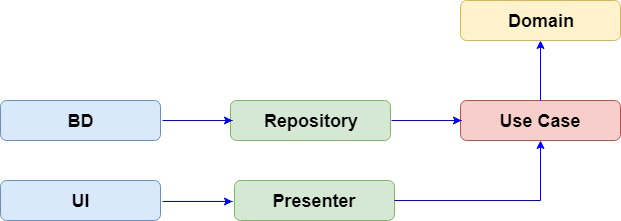
\includegraphics[scale=0.5]{ca_dep.png}
    \caption{General dependency diagram}
\end{figure}
\begin{itemize}
\item The domain layer (Entities) is independent of all layers.
\item The application layer (Usecase) depends on the domain layer and is independent of other layers. This layer prepares responses to
user queries using entities.
\item The adapters interface layer depends on the application(Usecase) layer.
This layer transmits the user request and the necessary data
to its processing at the Use Cases layer and retrieves the response and structure
for the User Interface component.
\item The user interface (UI) component of the "External technologies" layer
depends on the interface layer adapters through the Presenter an n
pass the user's request to it and retrieves the response.
\item The database component of the "External technologies" layer
allows the Use Case layer to retrieve data through a
Gateway(Repository) belonging to the Interface Adapter layer.

\end{itemize}
The following figure shows an example of a detailed dependency between
layers of the clean architecture pattern in the case of our application. These dependencies link a set of classes belonging to the different layers.
These classes realize the example of the functionality of displaying the list of
users.
\begin{figure}[H]%
    \center   
    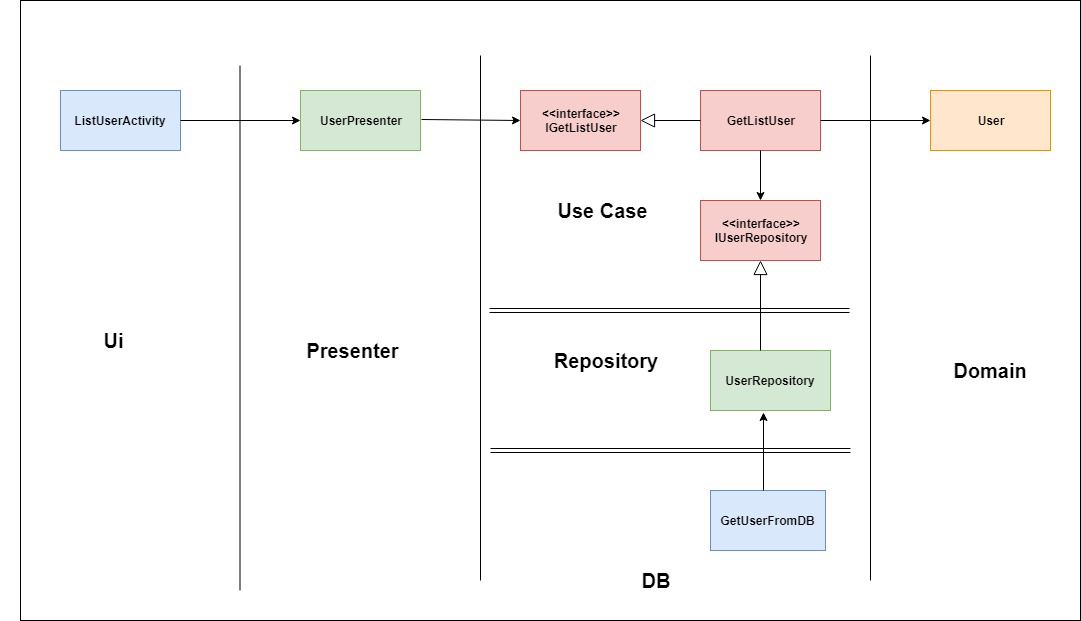
\includegraphics[scale=0.5]{ca_dep_detail.png}
    \caption{Detailed dependency diagram in case of functionality
print the list of users}
\end{figure}
According to the figure, the Interface Adapter layer (UserPresenter and UserRepository)
communicates (passing and retrieving data) with the Use layer
boxes by implementing or instantiating its IGetListUser and IUser-
Repository. These interfaces represent the "ports" of the Use Cases layer.
This example shows how we realized the principle of independence
from the core of the application of the technologies used. No instance of the
adapters interface layer or outer layer exists in the app's core.
\section{Dynamic view of the application}
In this section, we will describe the internal dynamic of our application using sequence diagrams and activity diagrams
\subsection{Detailed sequence diagram of the "register" use case}
The following figure illustrates the detailed sequence diagram of the use case
"register".
This use case starts with opening a registration interface
for the user. Then, the user enters his coordinates and confirms them.
The system displays an error message if the email already exists otherwise it redirects
the user to the home page. 
\begin{figure}[H]%
    \center   
    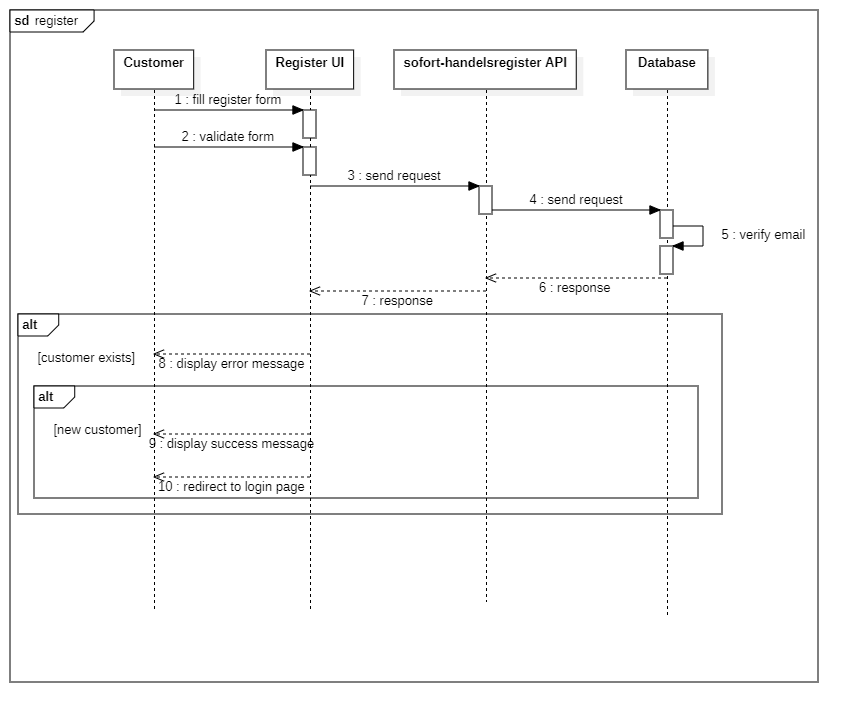
\includegraphics[scale=0.5]{seq_r.png}
    \caption{Detailed sequence diagram of the "register" use case}
\end{figure}
\subsection{Detailed sequence diagram of the "login" use case}
The following figure illustrates the detailed sequence diagram of the use case
"login".
This use case starts with opening a login interface
for the user. Then, the user enters his email and password then confirms them.
The system displays an error message if the email or the password is incorrect otherwise it redirects
the user to the home page.
the user may also choose to log in using a social media account ( Google, Facebook, LinkedIn, Xing), by taping the dedicated button to each social media which will redirect him to the interface provided by that specific social media API, the user will be redirected to the home interface upon successful social media login.
  \begin{figure}[H]%
    \center   
    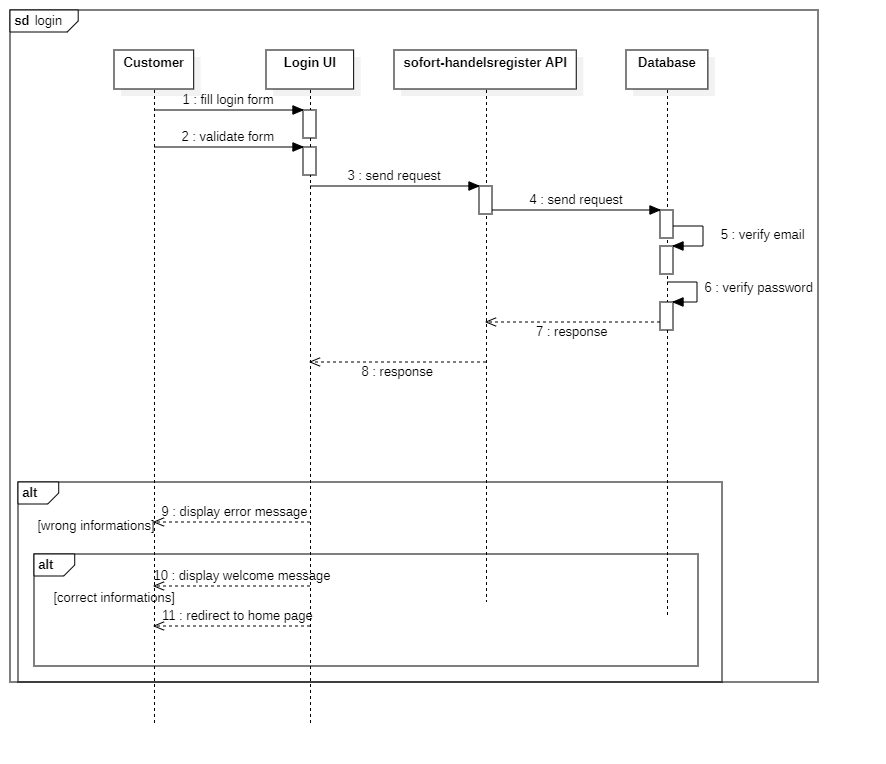
\includegraphics[scale=0.5]{seq_l.png}
    \caption{Detailed sequence diagram of the "login" use case}
\end{figure}
\begin{figure}[H]%
    \center   
    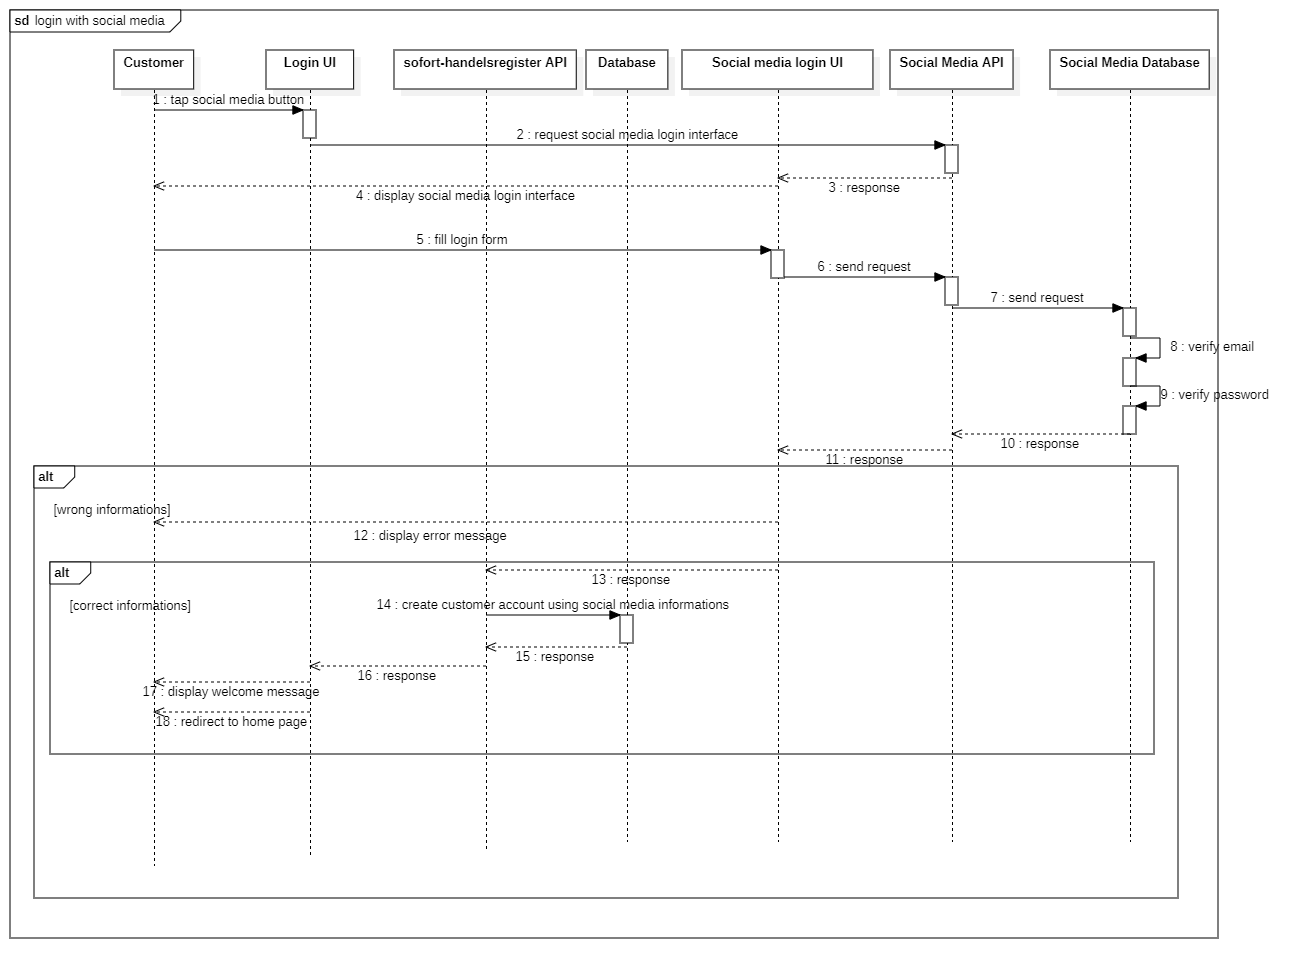
\includegraphics[scale=0.4]{seq_ls.png}
    \caption{Detailed sequence diagram of the "login with social media" use case}
\end{figure}
\subsection{Detailed sequence diagram of the "search company" use case}
The following figure illustrates the detailed sequence diagram of the use case
"search company".
This use case starts with opening an interface for the company's search for the user. Then the user enters the name of the wanted company's name or the first letters of its name, he may also add some filter to the results using a different interface (by state, zip code, legal form, capital, branch), upon confirming his request the interface will prompt an interactive list of results where the user may tap one of them to access more detailed information about it.
 \begin{figure}[H]%
    \center   
    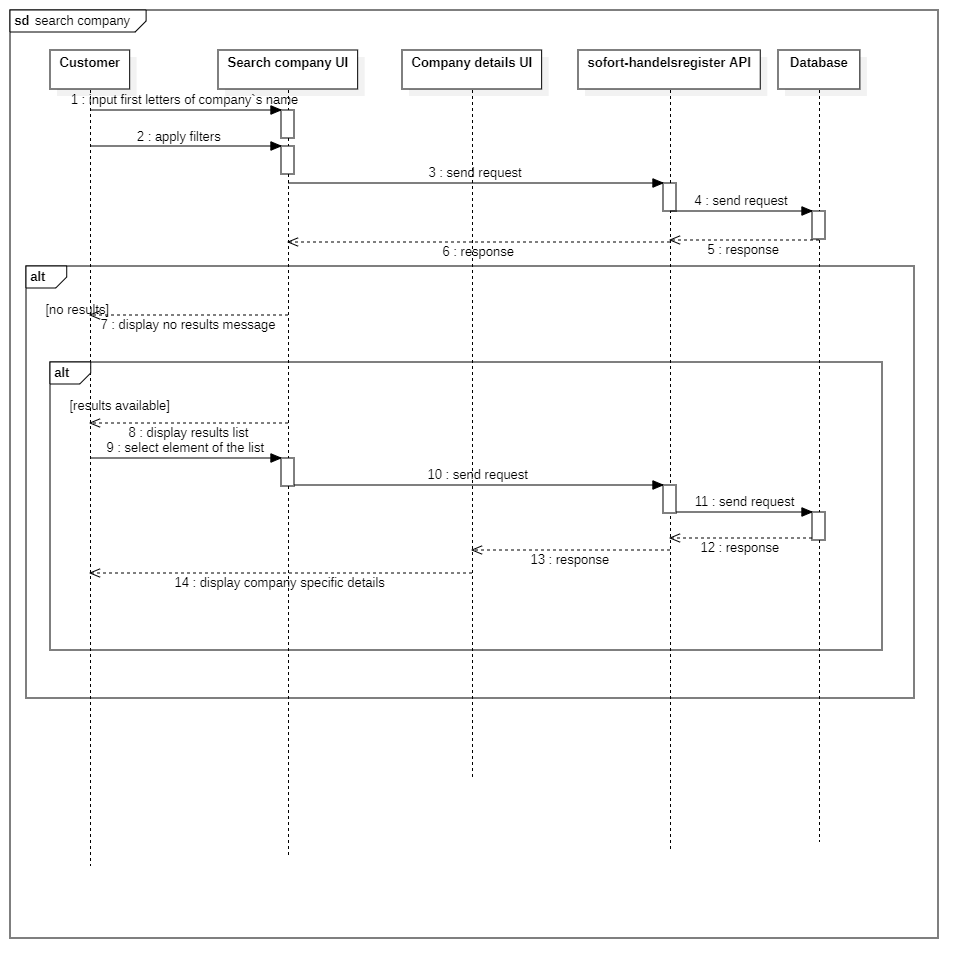
\includegraphics[scale=0.5]{seq_s.png}
    \caption{Detailed sequence diagram of the "search company" use case}
\end{figure}

\subsection{Detailed sequence diagram of the "follow company" use case}
The following figure illustrates the detailed sequence diagram of the use case
"follow company".
This use case starts with opening an interface containing specific company details for the user. Then the user may tap the follow button to add that company to his tracked companies list and start receiving notifications about it, these notifications may be deactivated later in the tracked companies interface.
\begin{figure}[H]%
    \center   
    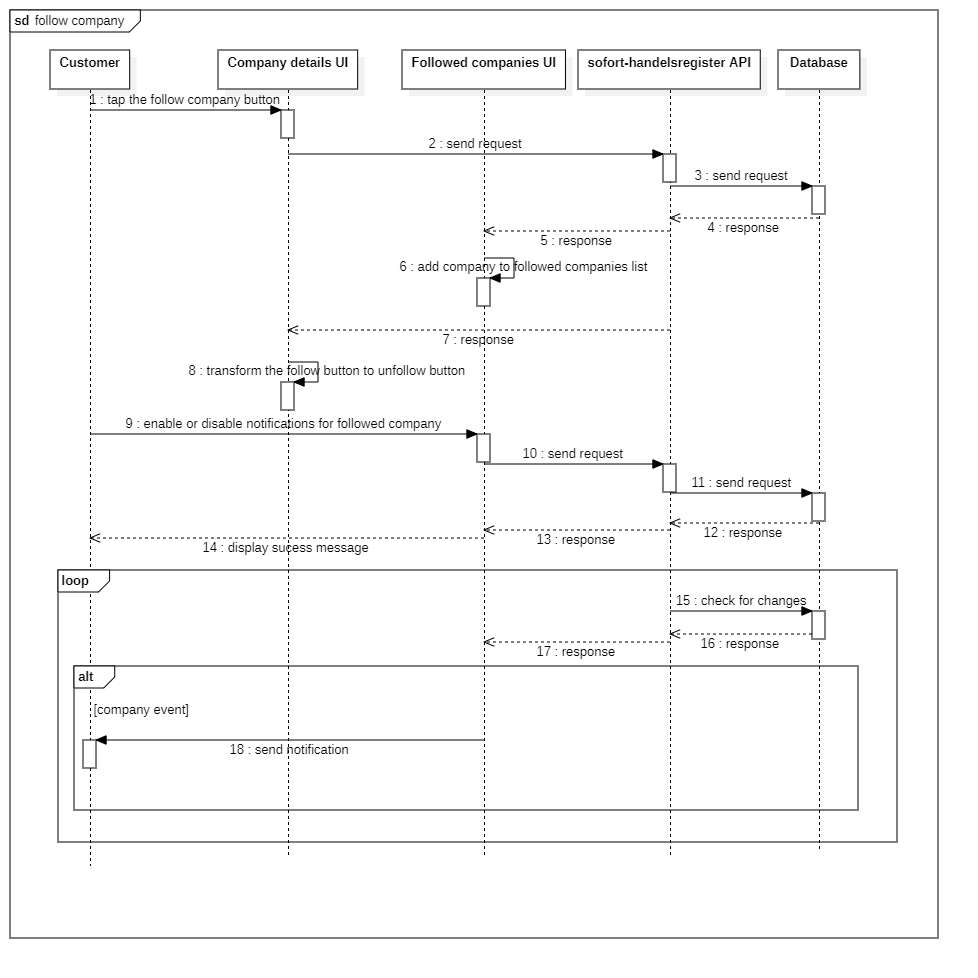
\includegraphics[scale=0.5]{seq_f.png}
    \caption{Detailed sequence diagram of the "follow company" use case}
\end{figure}
\subsection{Detailed sequence diagram of the "purchase documents" use case}
The following figure illustrates the detailed sequence diagram of the use case
"purchase documents".
This use case starts with opening an interface containing specific company details for the user. Then the user may scroll down to the documents section and add wanted documents to his cart, after that he may checkout and finalize his purchase process after filling in his credit card details. As a result, the purchased documents are added to the user's inventory interface and he may download them.
\begin{figure}[H]%
    \center   
    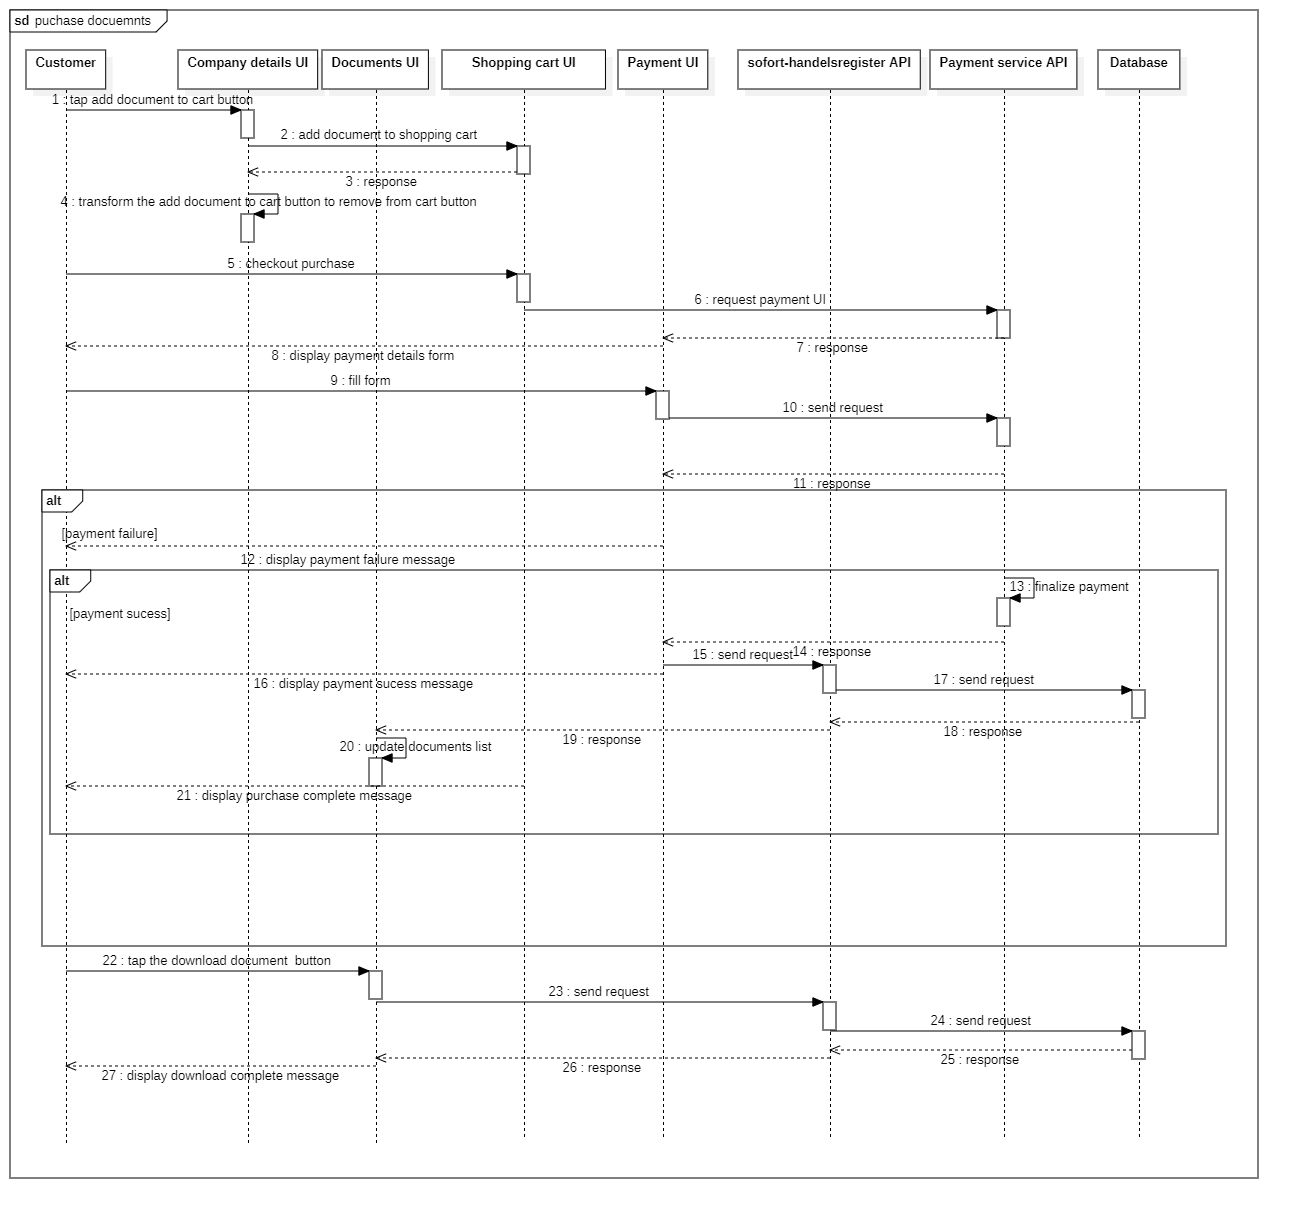
\includegraphics[scale=0.4]{seq_p.png}
    \caption{Detailed sequence diagram of the "purchase documents" use case}
\end{figure}
\section*{Conclusion}
This chapter presents one of the most important phases of the process of
development of a project: design subdivided into the overall design
and detailed design.\\
We presented the Clean Architecture architecture pattern and we
explained its application in our case. We have described the dynamic view
of the system through a set of sequence diagrams and diagrams
of activities.\\
The following chapter will deal with the realization of the project illustrated by screenshots of different interfaces. We will describe the environment of
work and the tools used too.